\newpage
\section{Электромагнитные волны}
\subsection{Свободное электромагнитное поле}
    Свободное поле --- это, иными словами, поле в пустом пространстве, описываемое уравнениями
    \begin{gather*}
        \rho(\vec{r}) = 0; \\
        \vec{j}(\vec{r}) = 0.
    \end{gather*}
    Уравнения Максвелла при таких условиях принимают вид
    \begin{gather}
        \rot\vec{E}(\vec{r}, t) = -\frac 1c \pard{\vec{H}}{t}; \label{free_rote} \\
        \Div\vec{E}(\vec{r}, t) = 0; \notag \\ 
        \rot\vec{H}(\vec{r}, t) = \frac 1c \pard{\vec{E}}{t}; \label{free_roth} \\
        \Div\vec{H}(\vec{r}, t) = 0. \notag
    \end{gather}
    Применим к уравнению (\ref{free_rote}) операцию ротора:
    \[
        \rot\rot\vec{E} = \grad\Div\vec{E} - \Delta\vec{E} = -\frac 1c \pard{\rot\vec{H}}{t}
        = -\frac 1{c^2}\pardd{\vec{E}}{t}.
    \]
    В силу равенства $\Div\vec{E} = 0$ это уравнение сводится к виду
    \[
        \frac 1{c^2} \pardd{\vec{E}}{t} - \Delta\vec{E} \equiv \Box\vec{E} = 0.
    \]
    Применяя операцию ротора к (\ref{free_roth}), получаем аналогичное уравнение
    \[
        \Box\vec{H} = 0.
    \]
    Применим калибровку Лоренца ($\frac 1c \pard{\phee}{t} + \Div\vec{A} = 0$), чтобы получить уравнения на потенциалы:
    \begin{gather*}
        \frac 1{c^2} \pardd{\phee}{t} - \Delta\phee = 0;\\
        \frac 1{c^2} \pardd{\vec{A}}{t} - \Delta\vec{A} = 0.
    \end{gather*}
    Как видно, в случае калибровки Лоренца уравнения на потенциалы имеют вид волновых уравнений, причём в частном случае свободного поля
    эти уравнения однородные (правая часть равна нулю, в общем случае там $4\pi\rho$ или $\frac{1}{c}4\pi\vec{j}$).

    В общем случае для описания потенциалов необходимы четыре независимых величины. Однако, в случае свободного поля оказывается,
    что в рамках калибровки Лоренца четыре величины избыточны, и можно выбрать более узкую калибровку, в которой $\phee = 0$.
    Сделаем такое добавочное калибровочное преобразование:
    \begin{gather*}
        \tilde{\phee} = \phee - \frac 1c \pard{\chi}{t};\\
        \tilde{\vec{A}} = \vec{A} + \nabla\chi
    \end{gather*}
    Подставим $\tilde{\phee}$ в условие калибровки Лоренца:
    \[
        \frac 1c \pard{\tilde{\phee}}{t} + \frac 1{c^2}\pardd{\chi}{t} + \Div\tilde{\vec{A}} - \Delta\chi = 0.
    \]
    Чтобы это условие сохранилось, наложим на функцию $\chi$ следующее условие:
    \begin{equation}
        \frac 1{c^2} \pardd{\chi}{t} - \Delta \chi = 0 \: \leftrightarrow \: \Box\chi = 0. \label{takie_chi}
    \end{equation}
    Среди таких функций $\chi$ таких, что выполнено (\ref{takie_chi}), найдем такую, что $\tilde{\phee} = 0$.
    \begin{note}
        В отличие от калибровки Лоренца, данная калибровка не является релятивистски инвариантной. То есть, перейдя в другую систему отсчёта,
        мы и там сможем занулить скалярный потенциал $\phee$, но найденная функция $\chi$ будет уже другой.
    \end{note}
    Далее все потенциалы подразумеваются с тильдами, хотя непосредственно тильды не пишутся.
    Запишем уравнения свободного поля в новой калибровке (далее все потенциалы подразумеваются с тильдами, хотя непосредственно тильды не пишутся):
    \begin{gather*}
        \vec{E} = -\frac{1}{c} \pard{\vec{A}}{t}; \:\: \Box\vec{E} = 0;\\
        \vec{H} = \rot\vec{A}; \:\: \Box\vec{H} = 0;\\
        \Div\vec{A} = 0; \:\: \Box\vec{A} = 0.
    \end{gather*}
    Уравнение на скалярный потенциал отсутствует, ведь зануляя его, мы как раз добивались упрощения системы уравнений,
    описывающих свободное поле.

\subsection{Плоские электромагнитные волны}
    Плоской волна называется в том случае, если в пространстве существует выделенное направление $X$, такое, что решения
    волновых уравнений зависят только от времени и координаты $X$, а от координат $Y$ и $Z$ не зависят. Уравнения таких волн имеют
    общий вид
    \begin{equation}
        \frac 1{c^2} \pardd{f}{t} - \pardd{f}{x} = 0, \label{wave_eq}
    \end{equation}

    где в качестве $f = f(x, t)$ может стоять какая-либо компонента векторов $\vec{E}$, $\vec{H}$ или $\vec{A}$.
    Решения (\ref{wave_eq}) имеют вид
    \[
        f(x, t) = f_1\brackets{t - \frac xc} + f_2\brackets{t + \frac xc},
    \]
    где $f_1, f_2$, вообще говоря, произвольные функции.

    Рассмотрим, как направлен векторный потенциал в такой волне. В одномерном случае условие $\Div\vec{A} = 0$
    равносильно условию $\pard{A_x}{x} = 0$. Тогда получаем, что
    \[
        \pard{A_x}{x} = 0 \: \Rightarrow \: \pardd{A_x}{x} = 0 \: \Rightarrow \: 
        (\textrm{с уч. (\ref{wave_eq}) для компоненты $A_x$}) \: \Rightarrow \: \pard{A_x}{t} = const(t) = -c\cdot E_x.
    \]
    Нас не интересуют не зависящие от времени решения, нас интересуют электромагнитные волны в
    пустом пространстве, где есть зависимость от времени. Поэтому положим эту константу $\pard{A_x}{t}$ равной нулю (подобно тому, как мы отсеиваем постоянное
    напряжение на входе осциллографа, анализируя синусоидальные колебания). Вместе с ней, в силу пропорциональности, обратится в ноль $E_x$.
    Также, $\pard{A_x}{t} = 0 \: \Rightarrow \: A_x = const = 0$ --- составляющую $A_x$ обратим в ноль на том же основании. То есть,
    векторный потенциал может быть выбран так, что $\vec{A} \perp \vec{e}_x \equiv \vec{n}$, где $\vec{n}$ --- направление распространения
    волны.

    Рассмотрим волну, распространяющуюся в положительном направлении (для отрицательного всё аналогично):
    \begin{gather*}
        \vec{A}(x, t) = \vec{A}(t - \frac xc); \\
        \vec{E} = -\frac 1c \pard{\vec{A}}{t} = -\frac 1c \brackets{\vec{A}}';\\
        \vec{H} = \rot\vec{A} = \sqbrk{\nabla\brackets{t - \frac xc} \times \brackets{\vec{A}}'} = \\ =
        -\frac 1c \sqbrk{\vec{e}_x \times \brackets{\vec{A}}'} = -\frac 1c \sqbrk{n \times \brackets{\vec{A}}'} = \vecp{n}{E}.
    \end{gather*}
    Заметим, что $\vec{H} \perp \vec{n}$, $\vec{E} \perp \vec{n}$, $\vec{H} \perp \vec{E}$.
    Более того, $\abs{\vec{H}} = \abs{\vec{E}}$.

    Энергия в плоской электромагнитной волне распространяется со скоростью света:
    \[
        \vec{S} = \frac c{4\pi}\vecp{E}{H}= \frac{c}{4\pi}\sqbrk{\vec{E} \times \vecp{n}{E}} = 
        \frac{c}{4\pi} E^2\vec{n} = cw\vec{n},
    \]
    \[
        \textrm{где } \: w = \frac{E^2 + H^2}{8\pi} = \frac{E^2}{4\pi} = \frac{H^2}{4\pi} \: \textrm{--- плотность энергии ЭМ волны.}
    \]
    Плотность потока импульса плоской волны равна
    \[
        \vec{g} = \frac{\vec{S}}{c^2} = \frac wc\vec{n}.
    \]

\subsection{Монохроматические плоские волны}
    В монохроматических волнах зависимость от времени связана происходит по закону синуса, то есть в уравнении (\ref{wave_eq}) 
    $f = \cos(\omega t + \alpha)$ или $f = \sin(\omega t + \alpha)$.
    В общем виде косинус будет удобно представить как действительную часть комплексной экспоненты, например,
    \[
        \vec{A}(x, t) = \re\braces{\vec{A}_0 \cdot e^{-i\omega\brackets{t - \frac{x}{c}}}} = 
        \re\braces{\vec{A_0}e^{-i\omega t + i\dotp{k}{r}}} = \re\braces{\vec{A}_0e^{-ik_ix^i}},
    \]
    где $\vec{A}_0 \perp \vec{e}_x \equiv \vec{n}$, $\vec{k} = \frac{\omega}c\vec{n}$.
    В силу линейности волновых уравнений вместо действительной части можно писать экспоненту полностью:
    \[
        \vec{A}(x, t) = \vec{A}_0e^{i\dotp{k}{r} - i\omega t}
    \]
    При такой записи
    \[
        \Div\vec{A} = 0 \: \Leftrightarrow \: \dotp{A}{k} = 0 \: \Leftrightarrow \: \vec{A} \perp \vec{k}
    \]
    Уравнения полей примут вид
    \begin{gather*}
        \vec{E} = -\frac 1c \pard{H}{t} = \frac{i\omega}c\vec{A};\\
        \vec{H} = \rot\vec{A} = i\vecp{k}{A} = \vecp{n}{E},
    \end{gather*}
    а условия на дивергенцию сведутся к условиям перпендикулярности:
    \begin{gather*}
        \Div\vec{E} = 0 \: \Leftrightarrow \: \dotp{k}{E} = 0;\\
        \Div\vec{H} = 0 \: \Leftrightarrow \: \dotp{k}{H} = 0.
    \end{gather*}

    Обсудим вопрос поляризации плоской монохроматической волны. Рассмотрим наблюдаемую часть волны --- электрическое поле:
    \begin{equation}
        \vec{E}(x, t) = \re\braces{\vec{E}_0e^{i\dotp{k}{r} - i\omega t}}. \label{elec_monochrom}
    \end{equation}
    $\vec{E}_0$ --- некоторый комплексный вектор. Выразим $\vec{E}_0$ через некоторый вектор $\vec{b}$, имеющий действительный квадрат, и фазу $\alpha$:
    \begin{gather*}
        \dotp{E_0}{E_0} = E_0^2 = \abs{E_0}^2\cdot e^{-2i\alpha};\\
        \dotp{E_0}{E_0}\cdot e^{2i\alpha} = \abs{E_0}^2 = \brackets{\vec{E}_0e^{i\alpha}}^2 = \abs{\vec{b}}^2;
        \vec{b} = \vec{E}_0e^{i\alpha}.
    \end{gather*}
    Подставим $\vec{E_0}$ в (\ref{elec_monochrom}):
    \[
        \vec{E}(x, t) = \re\braces{\vec{b}\cdot e^{i\dotp{k}{r} - i\omega t - i\alpha}}.
    \]
    Сам вектор $\vec{b}$, вообще говоря, комплексный. Запишем его в виде $\vec{b} = \vec{b}_1 + i\vec{b}_2$.
    \[
        \brackets{\vec{b}}^2 = b_1^2 - b_2^2 + 2i\dotp{b_1}{b_2} \in \R \: \Rightarrow \: \vec{b}_1 \perp \vec{b}_2.
    \]
    Направим векторы по осям $Y$ и $Z$: $\vec{b}_1 \sim \vec{e}_y$, $\vec{b_2} \sim \vec{e}_z$. В этом случае
    \begin{gather*}
        E_y(x, t) = b_1\cos\brackets{\vec{k}\cdot\vec{r} - \omega t - \alpha};\\
        E_z(x, t) =\pm b_2\cos\brackets{\vec{k}\cdot\vec{r} - \omega t - \alpha}.
    \end{gather*}
    Заметим теперь, что колебания электрического поля описывают эллипс в плоскости $Y-Z$:
    \[
        \brackets{\frac{E_y}{b_1}}^2 + \brackets{\frac{E_z}{b_2}}^2 = 1 \: \textrm{--- уравнение эллипса.}
    \]
    В общем случае монохроматическая волна имеет эллиптическую поляризацию. В частных случаях она может вырождаться в круговую ($b_1 = b_2$)
    или линейную ($b_1 = 0$ или $b_2 = 0$) поляризацию.
    
    Если излучение поляризовано не полностью или вообще не поляризовано, его представляют как совокупность волн с
    разным направлением $\vec{e}$ линейной поляризации:
    \begin{figure}[h]
        \centering{
            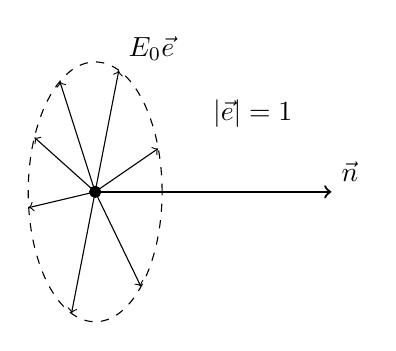
\begin{tikzpicture}
    \draw [black, dashed] (0, 0) ellipse (0.85cm and 1.65cm);
    \filldraw [black] (0,0) circle (2pt);
    \draw [->] (0, 0) -- (0.8, 0.55);
    \draw [->] (0, 0) -- (0.3, 1.54) node [anchor = south west] {$E_0\vec{e}$};
    \draw [->] (0, 0) -- (0.58, -1.2);
    \draw [->] (0, 0) -- (-0.3, -1.54);
    \draw [->] (0, 0) -- (-0.844, -0.2);
    \draw [->] (0, 0) -- (-0.77, 0.69);
    \draw [->] (0, 0) -- (-0.448, 1.4);
    \draw [->, thick] (0,0) -- (3,0) node [anchor = south west] {$\vec{n}$};
    \node [] at (2, 1) {$\left|\vec{e}\right| = 1$};
\end{tikzpicture}
        }
    \end{figure}
    Для нахождения интенсивности такого излучения применяют \textit{усреднение по поляризациям}. При вычисленях в таком случае
    неизбежны выражения вида  $\langle e_{\alpha}e_{\beta}\rangle$, которые могут быть представены как комбинация дельта-символа
    и вектора $\vec{n}$, так как это выделенное направление в задаче. В случае полной изотропии результат не зависел бы от направления
    и выражался только через дельта-символ.
    \[
        \langle e_{\alpha}e_{\beta}\rangle = a\delta_{\alpha\beta} + bn_{\alpha}n_{\beta}.
    \]
    Скалярные множители находятся из следующих условий:
    \begin{gather*}
        \langle e_{\alpha}e_{\alpha}\rangle = a\delta_{\alpha\alpha} + bn_{\alpha}n_{\alpha} = 3a+b = 1;\\
        \vec{e} \perp \vec{n} \: \Rightarrow \: \langle n_{\alpha} e_{\alpha}e_{\alpha}\rangle =
        an_{\alpha}\delta_{\alpha\beta} + bn_{\alpha}n_{\alpha}n_{\beta} = \\ =
        (a + b)n_{\beta} = 0 \: \Rightarrow \: a+b = 0.
    \end{gather*}
    Отсюда $a = -b = \frac{1}{2}$, и
    \[
        \boxed{\langle e_{\alpha}e_{\alpha}\rangle = \frac{1}{2} \brackets{\delta_{\alpha\beta} - n_{\alpha}n_{\beta}}}
    \]